\documentclass{article}%
\usepackage[T1]{fontenc}%
\usepackage[utf8]{inputenc}%
\usepackage{lmodern}%
\usepackage{textcomp}%
\usepackage{lastpage}%
\usepackage[head=40pt,margin=0.5in,bottom=0.6in]{geometry}%
\usepackage{graphicx}%
%
\title{\textbf{Frente Amplio inicia la lucha unitaria hacia la transición}}%
\author{RAFAEL LEÓN | @Rleon\_9}%
\date{27/11/2018}%
%
\begin{document}%
\normalsize%
\maketitle%
\textbf{URL: }%
http://www.el{-}nacional.com/noticias/politica/frente{-}amplio{-}inicia{-}lucha{-}unitaria{-}hacia{-}transicion\_261210\newline%
%
\textbf{Periodico: }%
EN, %
ID: %
261210, %
Seccion: %
Política\newline%
%
\textbf{Palabras Claves: }%
NO\_TIENE\newline%
%
\textbf{Derecho: }%
12, %
Otros Derechos: %
CONTEXTO, %
Sub Derechos: %
\newline%
%
\textbf{EP: }%
NO\newline%
\newline%
%
\textbf{\textit{“Es el comienzo de una etapa de reunificación de las fuerzas democráticas dispuestas a enfrentar la dictadura“, señala la coalición en el manifiesto “Venezuela libre”, que presentó en la UCV}}%
\newline%
\newline%
%
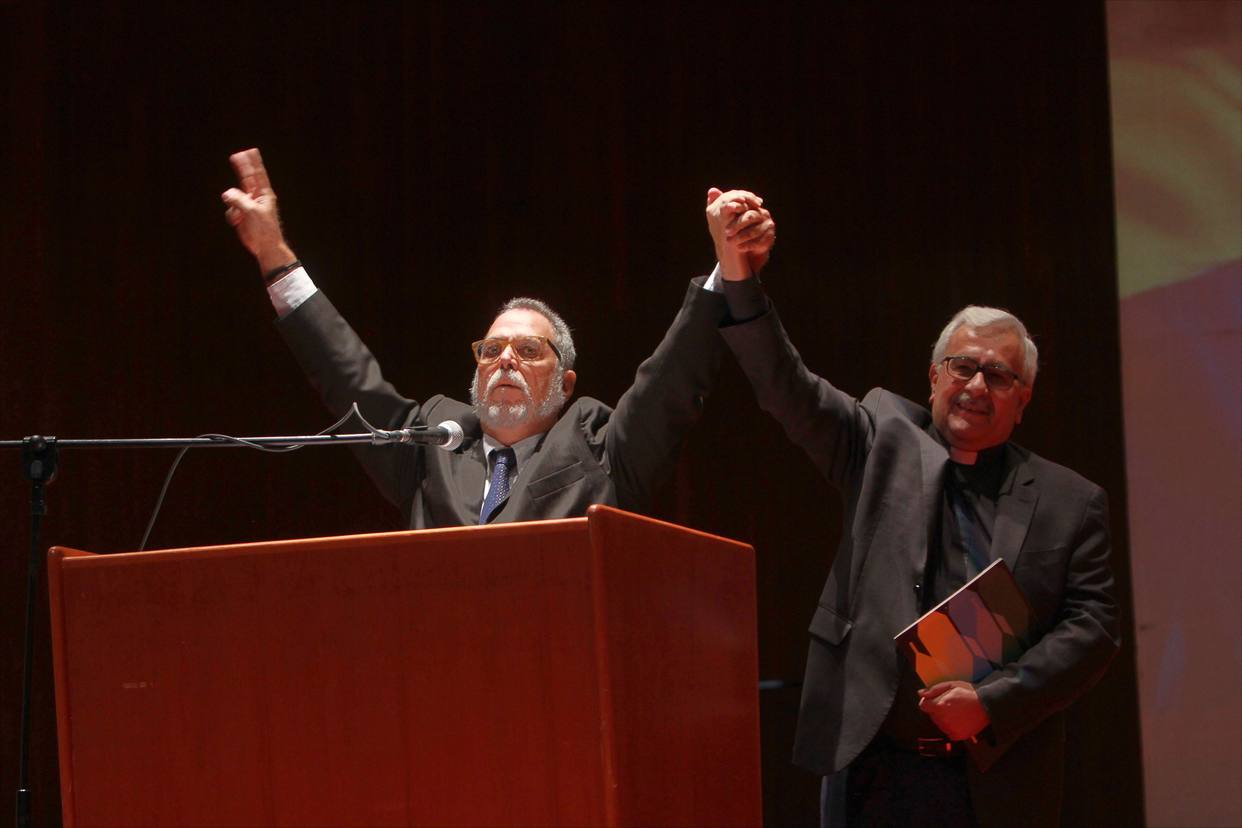
\includegraphics[width=300px]{140.jpg}%
\newline%
%
El Aula Magna de~la Universidad Central~de Venezuela fue el centro del comienzo de otra fase de la lucha unitaria hacia un gobierno de transición y la reinstitucionalización del país. “El Congreso Venezuela Libre marca el inicio de una etapa de reunificación de las fuerzas democráticas dispuestas a enfrentar la dictadura”, fue el acuerdo principal del manifiesto que el Frente Amplio presentó.%
\newline%
%
Dirigentes de gremios y sindicatos, rectores de universidades,~la Iglesia, empresarios, estudiantes y políticos asistieron al acto para respaldar las propuestas. También estuvieron diplomáticos de Colombia, Argentina, México, Estados Unidos, Francia, Polonia, Países Bajos y representantes de la delegación de~la Unión Europea.%
\newline%
%
Víctor Márquez, presidente de~la Asociación~de Profesores de~la UCV, y José Virtuoso, rector de~la Universidad CatólicaAndrés Bello, fueron los encargados de cerrar el acto con la lectura del documento “Venezuela libre”, que recoge las conclusiones de las más de 1.800 iniciativas planteadas por los representantes de los sectores que participaron en los debates en los congresos regionales.%
\newline%
%
“Es la hora del encuentro, de la lucha compartida, del trabajo en equipo. Todos estamos convocados a dar el todo por el todo. A los amigos de~la Asamblea Nacional~y de los partidos le hemos dicho: Confiamos en ustedes, pero esperamos mucho más de ustedes”, expresó Virtuoso minutos antes de que Márquez leyera el manifiesto en el que proponen un plan de transición pacífica y constitucional de la mano del Parlamento junto con los sectores democráticos del país previo al 10 de enero, fecha en la que vence el periodo del presidente Nicolás Maduro.%
\newline%
%
“Nos organizamos desde ahora en instancias tácticas, estratégicas y logísticas para darle cauce al creciente malestar social del pueblo venezolano –víctima de una terrible crisis humanitaria y de un brutal proceso de empobrecimiento generalizado– a través de la protesta pacífica de calle que aumente la presión sobre la dictadura y haga cesar la usurpación”, dice.%
\newline%
%
El Frente Amplio se comprometió a construir un “acuerdo nacional”, en el que queden establecidas las reglas de una transición “ordenada e inmediata que garantice la plena vigencia de~la Constitución”. También prometieron presentar un plan de políticas públicas para ejecutarlo en el momento de la reconstrucción nacional.%
\newline%
%
En el texto ponen a disposición la plataforma para coordinar los reclamos sociales y la defensa de la democracia, ambos puntos son considerados esenciales para generar el paso a la democrática.%
\newline%
%
“Tenemos la gran responsabilidad de la esperanza de todo un país y lo que verán en este acto es el comienzo de esta nueva etapa de lucha”, dijo en la apertura de la actividad Gerardo Blyde, coordinador de los congresos regionales. Aseguró que entrega un Frente Amplio “revitalizado” luego de casi nueve meses de su creación.%
\newline%
%
Al ex alcalde de Baruta le siguió el padre Luis Ugalde, ex rector de~la UCAB, quien se refirió a la urgencia de la unidad de todos los sectores. “Basta ya de la ruina del país. Todos ~debemos estar unidos en el rescate de~la Constitución~democrática, descaradamente violada por un poder ilegitimo que se declara supraconstitucional”.%
\newline%
%
El religioso agregó: “Venezuela está con dolores de parto y necesita renacer. La política, la economía, la sociedad nos encontramos en un solo abrazo de~la Venezuela~libre y plural”.%
\newline%
%
Le siguieron Elaisa Ferri, del Frente Amplio de Mujeres, y Marlon Díaz, presidente de~la Federación~de Centros Universitarios de~la Universidad~de Carabobo, quien celebró “la lucha democrática” que dieron hace dos semanas en su casa de estudio.%
\newline%
%
“Los venezolanos no se rinden a pesar de la persecución política. Resistimos con valentía. Ese es el mejor homenaje que podemos rendir a líderes como el concejal Fernando Albán”, recordó.%
\newline%
%
Luego habló Ángel Oropeza, integrante de~la Secretaria~del Frente Amplio, que llamó a la articulación de todas las fuerzas y a la consolidación de una unidad superior. Negal Morales (Acción Democrática), secretario de~la Asamblea Nacional, y los diputados Stalin Gonzalez (UNT) y Juan Miguel Matheus (Primero Justicia) expusieron las consideraciones políticas del congreso.%
\newline%
%
Matheus indicó que la agenda de lucha está marcada por el 10 de enero, día en que se agrava la crisis política debido a que Maduro se juramentará con el desconocimiento de la mayoría del país y de la comunidad internacional.%
\newline%
%
En el congreso se acordó una reunión entre el Legislativo y los delegados regionales del Frente Amplio para el 12 de diciembre, con el fin de discutir la posición que asumirán en enero.%
\newline%
%
Sergio Sánchez, representante del chavismo disidente y que compartió escenario con Sairam Rivas, estudiante y ex presa política que estuvo en el Sebin, contó: “Sairam, detenida en el periodo de gestión de Miguel Rodriguez Torres, y yo, que trabaje con él, estamos acá juntos dando una demostración de unidad”.%
\newline%
%
Rivas fue la encargada de entregar las conclusiones de los congresos regionales a la directiva de~la Asamblea Nacional~para que sean incluidas en los debates. “El Parlamento está llamado a desempeñar un importante papel constitucional frente al 10 de enero. Hacemos un llamado a unir esfuerzos entre todos los sectores para reinstitucionalizar al país, construir una democracia y recuperar Venezuela”, señaló.%
\newline%
%
Estrategia frente al 10{-}E%
\newline%
%
Omar Barboza, presidente de~la Asamblea Nacional, consideró que los sectores que desean un cambio en el país deben coincidir en una estrategia para afrontar la situación que se generará luego del 10 de enero. “Hemos dicho que desde el 10 de enero no habrá un presidente electo, por lo cual debemos convenir en una estrategia para enfrentar este nuevo reto. Esperamos hacerlo unidos”. Indicó que el papel de los parlamentarios será de apoyo legislativo al tomar en cuenta en los debates las conclusiones del congreso.%
\newline%
%
Negociación y condiciones%
\newline%
%
Henrique Capriles, ex gobernador de Miranda, dijo que la transición para lograr la salida de la crisis se debe hacer con acuerdos y negociación que terminen en una~convocatoria de elecciones libres y transparentes. “No es verdad que una transición política tenga que ser obligatoriamente por un escenario de fuerza. Tenemos que permitir que exista una puerta para que quienes son responsables de esto, salgan”, expresó al finalizar el congreso en el que estuvo sentado al lado de otros ex gobernadores, entre ellos Manuel Rosales y Liborio Guarulla.%
\newline%
%
\end{document}